\usetikzlibrary{arrows}
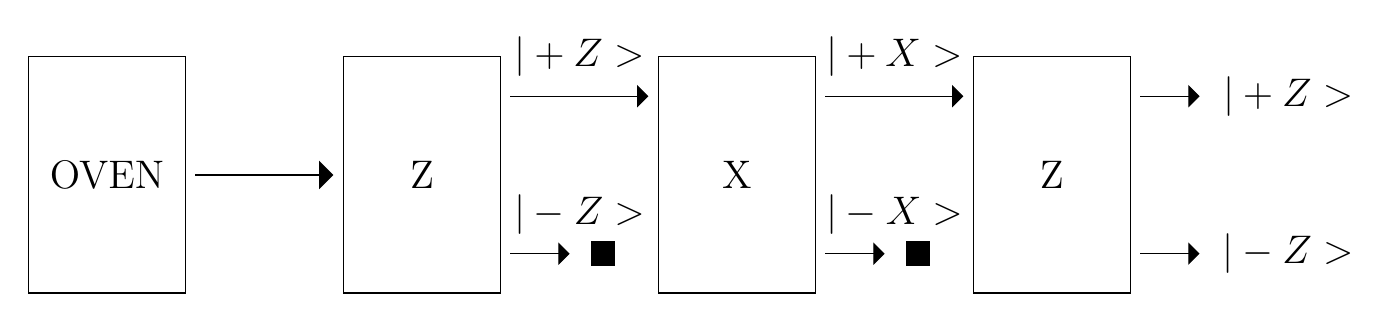
\begin{tikzpicture}

\draw  (-4,2.5) rectangle (-2,-0.5);
\draw  (0,2.5) rectangle (2,-0.5);
\node at (-3,1) {\Large OVEN};
\node at (1,1) {\Large Z};
\node (v1) at (-2,1) {};
\node (v2) at (0,1) {};
\node (v3) at (2,2) {};
\node (v5) at (2,0) {};
\node (v4) at (4,2) {};
\node (v6) at (3,0) {};

\draw [thick,-latex,   ->, -triangle 90] (v1) edge (v2);
\draw [-latex,   ->, -triangle 90] (v3) edge (v4);
\draw [-latex,   ->, -triangle 90] (v5) edge (v6);
\node at (3,2.5) {\Large $|+Z>$};
\node at (3,0.5) {\Large $|-Z>$};
\draw [o-*] (4,2.5) rectangle (6,-0.5);
\node (v7) at (6,2) {};
\node (v9) at (6,0) {};
\node (v8) at (8,2) {};
\node (v10) at (7,0) {};
\draw [o-*, -triangle 90] (v7) edge (v8);
\draw [o-*, -triangle 90] (v9) edge (v10);
\node at (7,2.5) {\Large $|+X>$};
\node at (7,0.5) {\Large $|-X>$};
\node at (5,1) {\Large X};
\draw [o-*, -triangle 90,fill] (3.15,0.15) rectangle (3.45,-0.15);
\draw  (8,2.5) rectangle (10,-0.5);
\draw[fill]  (7.15,.15) rectangle (7.45,-.15);
\node at (9,1) {\Large Z};
\node (v11) at (10,2) {};
\node (v13) at (10,0) {};
\node (v12) at (11,2) {};
\node (v14) at (11,0) {};
\draw [-triangle 90] (v11) edge (v12);
\draw [-triangle 90] (v13) edge (v14);
\node at (12,2) {\Large $|+Z>$};
\node at (12,0) {\Large $|-Z>$};
\end{tikzpicture}